\chapter{Conclusie}
In dit hoofdstuk wordt het laatste deel van de onderzoekscyclus behandeld, \qw{Deel 4: evalueren en adviseren} (zie figuur \ref{fig:ConclusieCyclus}).
Het eindresultaat wordt besproken en de uit eindelijk conclusie van het onderzoek wordt gedeeld.

\begin{graphic}
	\vspace{0.2cm}
	\captionsetup{type=figure}
	\caption{Deel 4 Verhoeven evalueren en adviseren afgeleid van \textit{Wat is Onderzoek?}}
	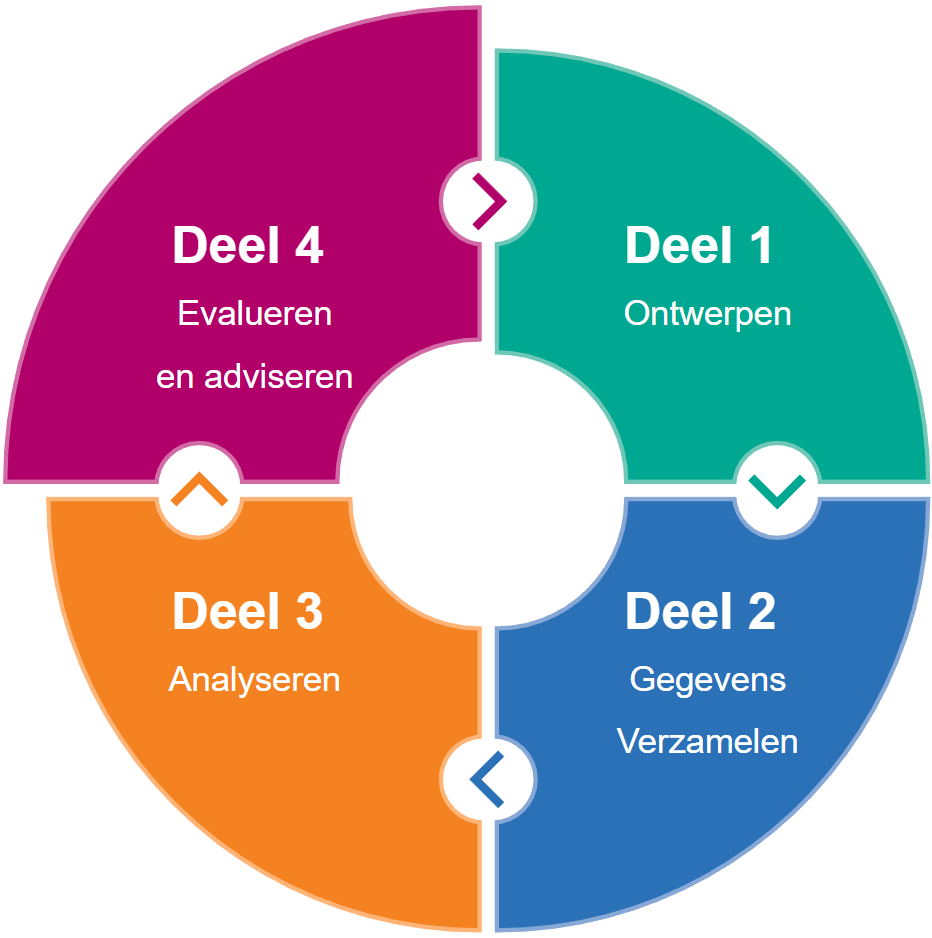
\includegraphics[scale=0.3]{img/EvaluerenCyclus.png}
	\label{fig:ConclusieCyclus}
	\vspace{0.2cm}
\end{graphic}

\whitespace
Het onderzoek is opgezet om een beter beeld te krijgen bij de eisen en wensen van de stakeholders die betrokken zijn bij de afstudeeropdracht.
Hierom is er gebruik gemaakt van de volgende hoofdvraag \qw{\textit{\MainQuestion}} en zijn de volgende deelvragen opgesteld om deze vraag te beantwoorden.
\newpage

\begin{center}
	\textit{Deelvraag 1: \SubquestionOne}
\end{center}

\whitespace
Binnen de afstudeeropdracht zijn er 4 verschillende stakeholders.
De beargumentatie voor de verschillende stakeholders en hun positie binnen het project is te vinden in sectie \ref{sec:Stakeholders}.
\begin{enumerate}
    \item{CEO}
    \item{Product owner}
    \item{Kleine bedrijven}
    \item{Afdeling R\&D}
\end{enumerate}
% Er zijn 4 verschillende stakeholders CEO, Product Owner, Kleine bedrijven en afdeling R\&D.

\begin{center}
	\textit{Deelvraag 2: \SubquestionTwo}
\end{center}

\whitespace
Om het systeem in beeld te brengen zijn er 2 tekeningen gemaakt die vervolgens vertaald zijn naar een digitale representatie.
Deze tekeningen zijn gemaakt met behulp van de architect van het huidige CMS Erwin Keuning en software engineer Kevin Snijder.
De tekeningen zijn terug te vinden in figuur \ref{fig:SystemArchitectureXSL} en \ref{fig:SystemArchitectureVue}.
Verder is er ook een versimpeld database model gemaakt die terug te vinden is in figuur \ref{fig:DatamodelCMS} en zijn er 5 randvoorwaarden opgesteld.
% Samen met de architect van het huidige CMS Erwin Keuning en R\&D software developer Kevin Sneider is het CMS inbeeld gebracht door middel van IT architecture scketching.
% Door dit proces zijn de huidige systemen duidelijker geworden en zijn er X Randwaarden voor het nieuwe systeem opgesteld.
% \todo[inline]{Betere tekst en randvoorwaarden opstellen}

\begin{center}
	\textit{Deelvraag 3: \SubquestionThree}
\end{center}

\whitespace
Er zijn 2 expertinterviews gehouden, een met Janny Reitsma en de andere Rob Douma.
Uit deze twee expertinterviews zijn verschillende knelpunten uitgekomen.
De knelpunten waar Janny tegen aanloopt staat beschreven in sectie \ref{sec:JannyInterview}, en die voor Rob staan beschreven in sectie \ref{sec:RobInterview}.

\begin{center}
	\textit{Deelvraag 4: \SubquestionFour}
\end{center}

\whitespace
Er is een ongeprioriteerde lijst met 15 functionele requirements verzameld.
De redenatie van de requirements zijn terug te vinden in sectie \ref{sec:Requirements} en de lijst van requirements is terug te vinden in bijlage \ref{appendix:Requirements}.

\begin{center}
	\textit{Deelvraag 5: \SubquestionFive}
\end{center}

\whitespace
Uit het resultaat van deelvraag 5 zijn er 6 Must haves, 6 Should haves, 1 Could haves en 2 Wont haves.
De redenatie van de prioritering is terug te vinden in sectie \ref{sec:Prioritering} en de complete lijst met geprioriteerde bijlage is terug te vinden in bijlage \ref{appendix:Requirements}.
Door het beantwoorden van deze vijf deelvragen kan de hoofdvraag beantwoord worden.

\begin{center}
	\textit{Hoofdvraag: \MainQuestion}
\end{center}

\whitespace
De kern functionaliteit van het nieuwe systeem is dat een eindgebruiker content kan plaatsen op de website.
De applicatie zal ontwikkeld worden binnen de randvoorwaarden vastgesteld zijn door het onderzoek.
Er zijn 15 functionele requirements (6 must-,6 should-, 1 could- en 2 wont haves) en 5 randvoorwaarden.
Door terug te kijken naar de doelstelling in sectie \ref{sec:Doelstelling} is het onderzoek doel behaald.

